\section{The Sound of sequences}
The On-line Encyclopedia of Integer Sequences (or OEIS) is an online database of number sequences taken from all branches of scientific investigation. It contains classical sequences such as the list of prime numbers or the sequence of Fibonacci numbers; or less known sequences taken from the solutions to mathematics problems, such as the ``number of planar graphs with n vertices''. The database was started in 1964 by mathematician Neil J. A. Sloane as a tool for identifying and understanding sequences. Today it includes more than 300 000 sequences.

Sequences can be analyzed mathematically, visualized as function graphs, or, as in this case, mapped onto sounds that can be heard. Besides revealing features of the sequence that are not obvious from just looking at the numbers, the resulting pieces of ``music'' are interesting in their own right, as we hope you agree from listening to the examples in this exhibit.

To convert a sequence of numbers to music -- to ``sonify'' it -- we use a simple algorithm. We map the sequence to the notes on a grand piano. This piano has 88 keys, and we number them 0, 1, ..., 87. We take the terms of the sequence, and add or subtract multiples of 88 until we get a number in the range 0 to 87.  In technical words, we read the sequence ``modulo 88''.

\begin{figure}[h]
\centering
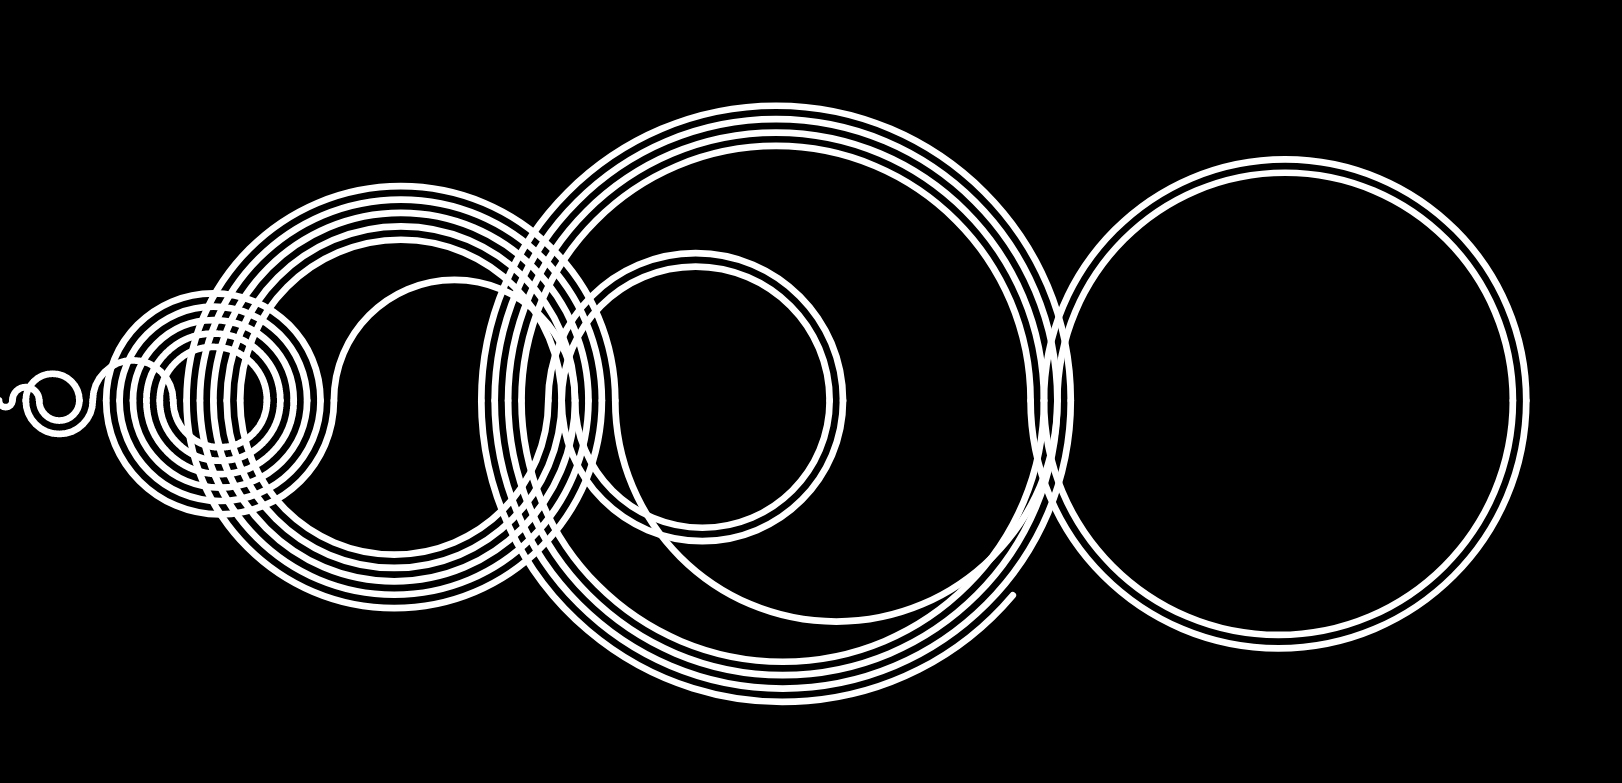
\includegraphics[width=0.7\textwidth]{SoundOfSequences}
\end{figure}

\vfill

Authors of the exhibit: Neil J. A. Sloane (data) and Eric Londaits for IMAGINARY (user interface). Text: Daniel Ramos (IMAGINARY).

References
The On-line Encyclopedia of Integer Sequences. \url{www.oeis.org}.

